\section{Method}

We study an asymmetric dense retriever with a full-depth document encoder and a compressed query encoder. Let $q$ denote a query and $d$ denote a document. The query tower is truncated to depth $L_q \in \{2,4\}$, while the document tower remains full depth and is frozen for all student experiments. For a text input $x$, each tower produces hidden states
$
H_r(x) \in \mathbb{R}^{T \times h}
$
with attention mask $m(x)$, where $r \in \{q,d\}$ indexes the query or document encoder.

\begin{figure}[t]
\centering
\resizebox{\columnwidth}{!}{% Standalone TikZ fragment for \input into the paper body.
% Assumes the document preamble already loads tikz and amsmath.
\begin{tikzpicture}[x=1cm,y=1cm, font=\small]
  % Palette kept muted for a short paper / systems-note aesthetic.
  \definecolor{queryfill}{RGB}{224,238,250}
  \definecolor{queryline}{RGB}{63,111,153}
  \definecolor{docfill}{RGB}{239,239,239}
  \definecolor{docline}{RGB}{110,110,110}
  \definecolor{scorefill}{RGB}{248,244,232}
  \definecolor{scoreline}{RGB}{154,124,56}

  % Query tower.
  \node[align=center] at (1.75, 6.55) {$q$};
  \node[align=center, text=queryline] at (1.75, 6.15) {$f_q^{(L_q)}$};
  \draw[rounded corners=1.5pt, line width=0.55pt, draw=queryline, fill=queryfill] (0.75,5.45) rectangle (2.75,5.95);
  \draw[rounded corners=1.5pt, line width=0.55pt, draw=queryline, fill=queryfill] (0.93,4.85) rectangle (2.57,5.35);
  \draw[rounded corners=1.5pt, line width=0.55pt, draw=queryline, fill=queryfill] (1.11,4.25) rectangle (2.39,4.75);
  \draw[rounded corners=1.5pt, line width=0.55pt, draw=queryline, fill=queryfill] (1.29,3.65) rectangle (2.21,4.15);
  \node at (1.75,4.55) {$\vdots$};
  \node[align=center, text=queryline] at (1.75,3.25) {$L_q=4$};
  \node[align=center] at (1.75,2.85) {$\hat z_q$};
  \draw[->, line width=0.65pt, draw=queryline] (1.75,3.55) -- (1.75,3.08);

  % Passage tower.
  \node[align=center] at (10.25, 6.55) {$d$};
  \node[align=center, text=docline] at (10.25, 6.15) {$f_d^{(L_d)}$};
  \draw[rounded corners=1.5pt, line width=0.55pt, draw=docline, fill=docfill] (9.25,5.45) rectangle (11.25,5.95);
  \draw[rounded corners=1.5pt, line width=0.55pt, draw=docline, fill=docfill] (9.07,4.95) rectangle (11.43,5.35);
  \draw[rounded corners=1.5pt, line width=0.55pt, draw=docline, fill=docfill] (8.89,4.45) rectangle (11.61,4.85);
  \draw[rounded corners=1.5pt, line width=0.55pt, draw=docline, fill=docfill] (8.71,3.95) rectangle (11.79,4.35);
  \draw[rounded corners=1.5pt, line width=0.55pt, draw=docline, fill=docfill] (8.53,3.45) rectangle (11.97,3.85);
  \draw[rounded corners=1.5pt, line width=0.55pt, draw=docline, fill=docfill] (8.35,2.95) rectangle (12.15,3.35);
  \node at (10.25,4.45) {$\vdots$};
  \node[align=center, text=docline] at (10.25,2.55) {full depth, frozen};
  \node[align=center] at (10.25,2.15) {$\hat z_d$};
  \draw[->, line width=0.65pt, draw=docline] (10.25,2.85) -- (10.25,2.35);

  % Shared scoring block.
  \draw[rounded corners=2pt, line width=0.7pt, draw=scoreline, fill=scorefill] (4.35,2.45) rectangle (7.65,4.35);
  \node[align=center, text=scoreline] at (6.0,3.65) {similarity score};
  \node[align=center] at (6.0,3.05) {$s(q,d)=\dfrac{\langle \hat z_q,\hat z_d\rangle}{\tau}$};
  \node[align=center, text=scoreline] at (6.0,2.7) {$\tau$ is fixed during evaluation};

  % Connectors.
  \draw[->, line width=0.65pt, draw=queryline] (2.21,2.85) -- (4.35,3.35);
  \draw[->, line width=0.65pt, draw=docline] (9.79,2.15) -- (7.65,3.35);

  % Top annotation.
  \node[align=center, text=black] at (6.0,6.9) {asymmetric dense retriever};
  \node[align=center] at (6.0,6.5) {$L_q \ll L_d,\qquad \text{document tower frozen}$};
\end{tikzpicture}
}
\caption{Asymmetric dense retrieval setup used throughout the student experiments. The query tower is truncated to depth $L_q$, while the document tower remains full-depth and frozen. Similarity is computed by scaled inner product over normalized embeddings.}
\label{fig:architecture}
\end{figure}

We pool hidden states with a low-cost operator $p_\rho(\cdot)$, where $\rho \in \{\mathrm{cls}, \mathrm{mean}\}$. The pooled vector is optionally transformed by a query-side projection head $g_\phi$ and then $\ell_2$-normalized:
\begin{align}
z_q(q) &= \mathrm{norm}\!\left(g_\phi\!\left(p_{\rho_q}\!\left(H_q(q), m(q)\right)\right)\right), \\
z_d(d) &= \mathrm{norm}\!\left(p_{\rho_d}\!\left(H_d(d), m(d)\right)\right).
\end{align}
In the symmetric teacher, the same backbone is used on both sides; in the asymmetric students, only the query encoder is truncated and only the query side may use a projection head.

Retrieval scores are scaled inner products:
\begin{equation}
s(q,d) = \alpha\, z_q(q)^\top z_d(d), \qquad \alpha = \exp(\tau),
\end{equation}
where $\tau$ is a learned log-temperature. This matches the study setup: normalized embeddings, inner-product similarity, and a learned scalar scale parameter.

Training uses an in-batch contrastive objective over positive query--document pairs. For a batch $\{(q_i, d_i^+)\}_{i=1}^B$, the logits are
\begin{equation}
\ell_{ij} = s(q_i, d_j^+),
\end{equation}
and the loss is
\begin{equation}
\mathcal{L}_{\mathrm{ctr}} = -\frac{1}{B}\sum_{i=1}^B \log \frac{\exp(\ell_{ii})}{\sum_{j=1}^B \exp(\ell_{ij})}.
\end{equation}
This is the only training signal for the baseline student and teacher fine-tuning runs.

When distillation is enabled, the student is regularized to match a frozen teacher similarity distribution over the same batch. Let $\ell^{S}_{ij}$ and $\ell^{T}_{ij}$ denote student and teacher logits. With distillation temperature $T$, the per-query distributions are
\begin{equation}
p^{S}_{i} = \mathrm{softmax}\!\left(\ell^{S}_{i\cdot}/T\right), \qquad
p^{T}_{i} = \mathrm{softmax}\!\left(\ell^{T}_{i\cdot}/T\right),
\end{equation}
and the distillation term is
\begin{equation}
\mathcal{L}_{\mathrm{KL}} = \frac{T^2}{B}\sum_{i=1}^B \mathrm{KL}\!\left(p^T_i \,\|\, p^S_i\right).
\end{equation}
The total objective is
\begin{equation}
\mathcal{L} = \mathcal{L}_{\mathrm{ctr}} + \lambda_{\mathrm{distill}} \mathcal{L}_{\mathrm{KL}},
\end{equation}
with $\lambda_{\mathrm{distill}} = 0$ for non-distilled runs.

Online cost is decomposed into query encoding and approximate or exact search:
\begin{equation}
T_{\mathrm{e2e}}(q) = T_{\mathrm{encode}}(q) + T_{\mathrm{search}}(q).
\end{equation}
In our measurements, $T_{\mathrm{encode}}$ is batch-size-1 query encoding latency and $T_{\mathrm{search}}$ is FAISS search latency against a fixed corpus index. We report p50 and p95 over a fixed query sample and separate the corpus indexing cost from query-time cost so the systems tradeoff is explicit.
